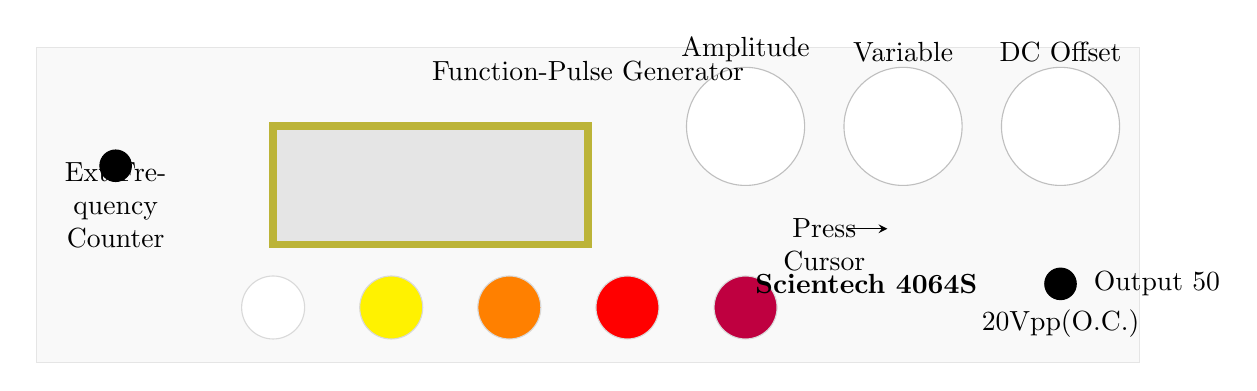
\begin{tikzpicture}[
    knob/.style={circle, draw=gray!50, fill=white, minimum size=15mm},
    button/.style={circle, draw=gray!30, fill=#1, minimum size=8mm},
    port/.style={circle, draw=black, fill=black, minimum size=4mm}
]
    % Main panel background
    \fill[gray!5] (0,0) rectangle (14,4);
    \draw[gray!20] (0,0) rectangle (14,4);
    
    % LCD Display
    \fill[black!10] (3,1.5) rectangle (7,3);
    \draw[yellow!70!black, line width=1mm] (3,1.5) rectangle (7,3);
    
    % Left port (Counter)
    \node[port] at (1,2.5) {};
    \node[text width=2cm, align=center] at (1,2) {Ext Frequency\\Counter};
    
    % Knobs on right side
    \node[knob] (amp) at (9,3) {};
    \node[above] at (9,3.7) {Amplitude};
    
    \node[knob] (var) at (11,3) {};
    \node[above] at (11,3.7) {Variable};
    
    \node[knob] (dc) at (13,3) {};
    \node[above] at (13,3.7) {DC Offset};
    
    % Output port
    \node[port] at (13,1) {};
    \node[right] at (13.3,1) {Output \SI{50}{\ohm}};
    \node[text width=2cm, align=center] at (13,0.5) {20Vpp(O.C.)};
    
    % Control buttons
    \node[button=white] at (3,0.7) {};
    \node[button=yellow] at (4.5,0.7) {};
    \node[button=orange] at (6,0.7) {};
    \node[button=red] at (7.5,0.7) {};
    \node[button=purple] at (9,0.7) {};
    
    % Title text
    \node[align=center] at (7,3.7) {Function-Pulse Generator};
    
    % Brand name
    \node[right] at (9,1) {\textbf{Scientech 4064S}};
    
    % Small cursor icon
    \path (10,1.5) node[align=center] {Press\\Cursor};
    \draw[->,>=stealth] (10.3,1.7) -- (10.8,1.7);
\end{tikzpicture}